\section{Assignment 7}
\subsection{Feature selection}

Before solving the clusterization problem we decided to do some empirical feature selection to get more interpretable and more clear-cut data structure. 
After some attempts we have choosen:
\begin{itemize}
	\item
	Channel-type nominal features
	
	\begin{itemize}
		\item
		\texttt{data\_channel\_is\_lifestyle}, \\
		\texttt{data\_channel\_is\_entertainment}, \\ 
		\texttt{data\_channel\_is\_bus}, \\ 
		\texttt{data\_channel\_is\_socmed}, \\
		\texttt{data\_channel\_is\_tech}, \\
		\texttt{data\_channel\_is\_world} (all are logical).
		
		\item
		\texttt{channel} (numeric from 0 to 6)
	\end{itemize}
	\item
	Some characteristics of words that article is composed of, it's title and it's keywords
	
	\begin{itemize}
		\item
		\texttt{n\_tokens\_title}, \\
		\texttt{n\_tokens\_content}, \\
		\texttt{n\_unique\_tokens}, \\
		\texttt{average\_token\_length}, \\
		\texttt{num\_keywords} (numeric).
	\end{itemize}
\end{itemize}

We have also logarithmed all log-normal features.
Unlike data filtering in previous assignments we decided to not to delete zero-length articles as to classify them as individual cluster.


\subsection{K-Means Clustering}

First of all we have plotted PCA-plot of our data, which is shown in Figure \ref{fig:k-means}. One can also find in this Figure clusterization results   when splitting data in 3,4 or 7 non overlapping parts.

Then we applied the built-in function \texttt{kmeans} with parameters $k=3,4,7$ and multi-start with $\texttt{nstart = 100}$, the results of this clusterization are presented in Figure \ref{fig:k-means}.
We should notice that the left-bottom cluster in all plots is rather far from the other clusters. During the data analysis we have found out that these points match zero-length articles.  

\begin{figure}[h]
	\centering
	\begin{minipage}[h]{0.49\linewidth}
		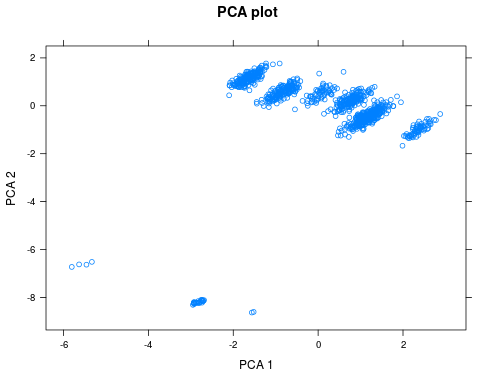
\includegraphics[width=\linewidth]{images/pcaplot_km}
	\end{minipage}
	\hfill
	\begin{minipage}[h]{0.49\linewidth}
		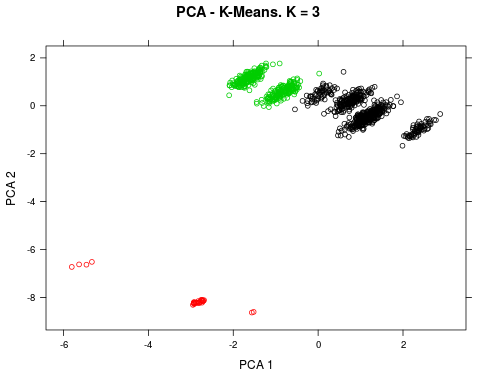
\includegraphics[width=\linewidth]{images/kmean3}
	\end{minipage}
	\begin{minipage}[h]{0.49\linewidth}
		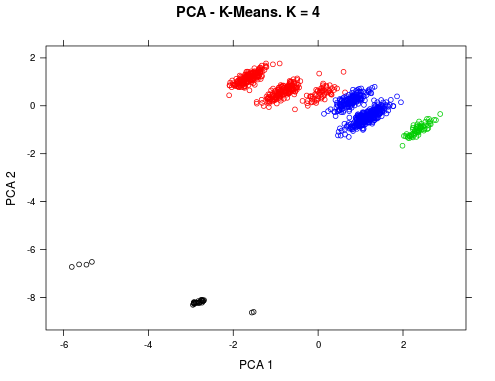
\includegraphics[width=\linewidth]{images/kmean4}
	\end{minipage}
	\hfill
	\begin{minipage}[h]{0.49\linewidth}
		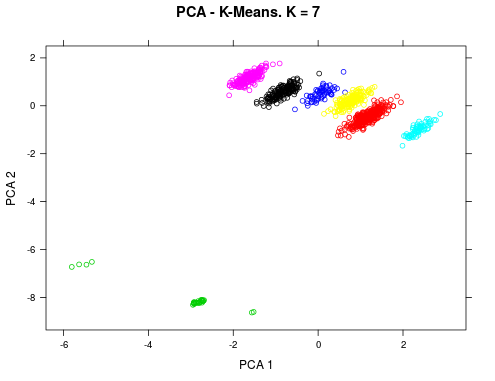
\includegraphics[width=\linewidth]{images/kmean7}
	\end{minipage}
	\caption{PCA plot without clusterization (a), with k-means clusterization with $k=3,4,7$}
	\label{fig:k-means}
\end{figure} 

As we know, k-means method is minimizing the value of total within-cluster sum of squares distance to cluster mean. 
In order to find the optimum number of clusters, we have built plot 
`total within-cluster sum of squares' to `number of clusters'  Choosing the right number of clusters for a clusterization problem is a rather difficult task. So to get some more intuition of what is really happening under the hood of K-means algorithm we have plotted the dependence of `total within-cluster sum of squares' to `number of clusters' (see Figure {\ref{fig:totalwithin-to-k}). This graph is often mentioned in connection of an `elbow' rule, which says that we should prefer the number of cluster equal to the  point on the x-axis, where this graph makes abrupt turn. 
	
So in our case this `silver bullet' rule says that we chould have either 7 or 8 clusters, and this seems rather  reasonable, especially when one take into account the appearance of the charts  (see Figure {\ref{fig:totalwithin-to-k}).
	
	\begin{figure}[h]
		\centering
		\begin{minipage}[h]{0.49\linewidth}
			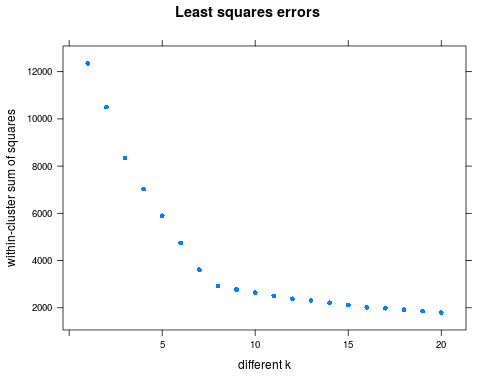
\includegraphics[width=1.2\linewidth]{images/totalwithin}
		\end{minipage}
		\caption{Dependence between `total within-cluster sum of squares' and `number of clusters'}
		\label{fig:totalwithin-to-k}	
	\end{figure}
	
	As we can see from the plot, the optimal number of clusters is about 7 (or 8, if we want to divide left-bottom cluster into two parts).
	
The other good method for choosing the number of clusters is the one called Hartigan’s Index
\begin{equation}
H_K =  \left(\dfrac{W_K}{W_{K+1}} - 1\right) \left(N-K-1\right)
\end{equation}
where $ N $ is equal to the whole number of entities, $ K $ is the number of clusters and $ W_K $ - is the total within-cluster sum of squares. 

So we have checked also this rule and plot this index relating to number of clusters. One could see the result in Figure \ref{fig:hartigan_index}.

\begin{figure}[h]
	\centering
	\begin{minipage}[h]{0.49\linewidth}
		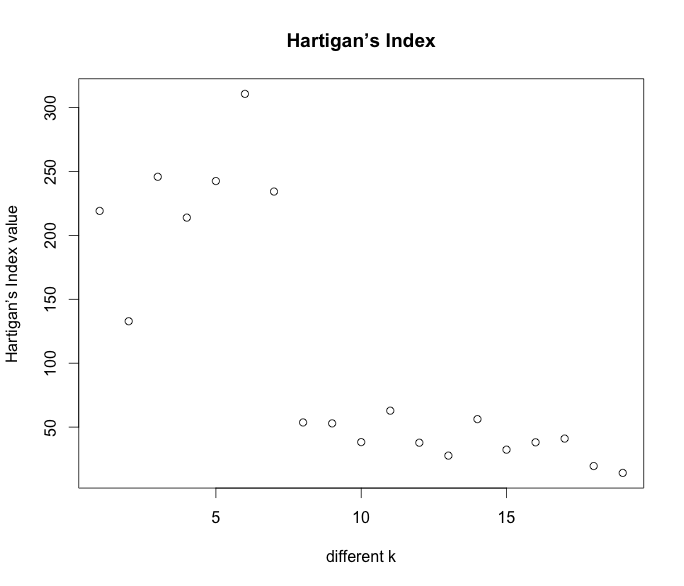
\includegraphics[width=1.2\linewidth]{images/hartigan_index.png}
	\end{minipage}
	\caption{Dependence between `Hartigan's index' and `number of clusters'}
	\label{fig:hartigan_index}	
\end{figure}

In \cite{CCODA_Mirkin} it is said that one should choose a very first $ k $, which is less then $ 10 $.  But we see here, that there is no any value of k in range from 1 to 20 that could be  choosen by this rule. So in our opinion this method needs some fine-tuning and more experiments.

One could also check the silhoulette index which we have plotted for every $ k $ in a same range as above. This plot is available in Figure \ref{fig:silhoulette_index}.
	

\begin{figure}[h]
	\centering
	\begin{minipage}[h]{0.49\linewidth}
		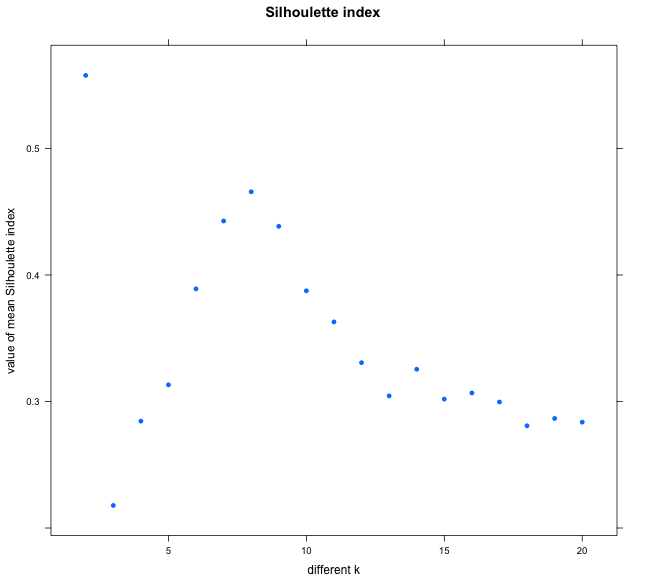
\includegraphics[width=1.2\linewidth]{images/silhoulette_index.png}
	\end{minipage}
	\caption{Dependence between `silhoulette' and `number of clusters'}
	\label{fig:silhoulette_index}	
\end{figure}

It also indicates that 8 clusters is the best possible choice.



\subsection{Nearest Neighbor clustering with MST}
	In this part of the assigment we have performed cluserting that is based on the minimal spaning tree algorithm. 
	We have used the Prima's algorithm to construct the Minimum Spanning Tree (aka MST further) of a complete, weighted and undirected graph, where entities of the dataset serve as vertexes.  To compute the weight of each edge we have found the distancies between the every pair of vertexes. MST is presented in Figure \ref{fig:mst_whole}.

\begin{figure}[h]
	\centering
	\begin{minipage}[h]{0.8\linewidth}
\includegraphics[width=\linewidth]{images/mst_whole.pdf}
	\end{minipage}	
	\caption{Minimum Spanning Tree of dataset.}
	\label{fig:mst_whole}	
\end{figure}	
	
	From the resulting MST we will delete $k-1$ edges with the greatest weights to obtain totally $k$ strongly connected components, aka  $k$ clusters. 
	
	One could see that  clustering with $k=7$ is more natural for our dataset, so we have  applied the aforementioned  method with number of cluster equal to  $k = 7$. So the graph one could see in Figure \ref{fig:mst_whole_removed_heaviest}  includes $7$ connected components (clusters).  The final clustering that was derived from MST algorithm is also shown in different colours in the Figure \ref{fig:mst_clusters_splitted}.

\begin{figure}[h]
	\centering
	\begin{minipage}[h]{0.8\linewidth}
\includegraphics[width=\linewidth]{images/mst_whole_removed_most_heaviest.pdf}
	\end{minipage}
	\caption{Graph of data after removing the $k=7$ heaviest edges from Minimum Spanning Tree.}
	\label{fig:mst_whole_removed_heaviest}	
\end{figure}	

\begin{figure}[h]
	\centering
	\begin{minipage}[h]{0.8\linewidth}
\includegraphics[width=\linewidth]{images/mst_clusters_splitted.pdf}
	\end{minipage}
	\caption{Clustering via k-Nearest Neighbourhood method with Minimum Spanning Tree.}
	\label{fig:mst_clusters_splitted}	
\end{figure}	

 To compare both method we have used  the mean Silhouette Coefficient, which is calculated as $\frac{(b - a) }{\max(a, b)}$ where the parameters calculated for each sample are mean intra-cluster distance (a) and mean nearest-cluster distance (b).  The mean Silhouette Coefficient for K-Means with $k = 7$ is equal to $0.44$ and for the Single Linkage Clustering with MST is equal to $0.01$. Thus we can conclude that clustering performance is better via K-Means method.
 
 This conclusion is also supported by the textbook \cite{CCODA_Mirkin}. 



